\section{Experiments}\label{experiments}
In this section, we empirically compare the performance of DMF with the classic centralized MF models, we also study the effects of parameters on model performance. 

\subsection{Setting}
We first describe the datasets, metrics, and comparison methods we use during our experiments. 

\textbf{Datasets.} We use two real-world datasets, i.e., \emph{Foursquare} and \emph{Alipay}. %, as shown in Table \ref{dataset}.
\emph{Foursquare} is a famous benchmark dataset for evaluating a POI recommendation model \cite{yang2016participatory}. 
%We randomly select 100 cities from the original dataset, and further remove the users and items that have less then 200 interactions\footnote{The reason that we sample a small dataset is that}. 
We randomly choose two cities for each country from the original dataset, and further remove the users and POIs that have too few or too many interactions\footnote{The reason we sample a small dataset is: we mock decentralized learning during our experiments, that is, there will be $2I \times \mathbb{R}^{K\times{}J}$ POI (global and local) latent matrices in total, which actually is not a small scale.}. 
%\emph{Alipay} is the biggest third-party online payment platform in China, through which users are able to delivery both online and offline payment. 
Our \emph{Alipay} dataset is sampled from user-merchant offline check-in records during 2017/07/01 to 2017/07/31, and we also perform similar preprocess on it. 
Table \ref{dataset} shows the statistics after process for both datasets, with which we randomly sample 90\% as training set and the rest 10\% as test set. 

\textbf{Metrics.} 
% We adopt three metrics that belong to two types to evaluate our model performance. 
% Root Mean Square Error (RMSE) is frequently used to evaluate the overall prediction performance of MF \cite{mnih2007probabilistic,jamali2009trustwalker,koren2009matrix}, and it it defined as 
% \begin{equation}
% RMSE=\sqrt{\frac{1}{|\tau|}\sum\limits_{(i,j) \in \tau}{(r_{ij}-\hat{r_{ij}})}^2},
% \end{equation}
% where $|\tau|$ is the number of predictions in the test dataset $\tau$. 
We adopt two metrics to evaluate our model performance, i.e., $P@k$ and $R@k$, which are commonly used to evaluate POI recommendation performance \cite{cheng2012fused,gao2015content}. 
For user $i$, they are defined as
\begin{equation}\nonumber\small
	P@k=\frac{|S^T_i \cap S^R_i|}{k},~~~
% \end{equation} 
% \begin{equation}\nonumber
	R@k=\frac{|S^T_i \cap S^R_i|}{|S^T_i|},
\end{equation} 
where $S^T_i$ denotes the visited POI set of user $i$ in the test data, and $S^R_i$ denotes the recommended POI set of user $i$ which contains $k$ POIs. 


\begin{table}
\centering
\caption{Dataset statistics.}
%\vskip -0.15in
\label{dataset}
\begin{tabular}{|c|c|c|c|c|}
  \hline
  Dataset & \#user & \#item & \#rating & \#cities \\
  \hline
  \hline
  \emph{Foursquare} & 6,524 & 3,197 & 26,186 & 117 \\
  \hline
  \emph{Alipay} & 5,996 & 7,404 & 18,978 & 298 \\
  \hline
\end{tabular}
%\vskip -0.15in
\end{table}

\textbf{Comparison methods.} 
Our proposed DMF framework is a novel decentralized algorithm for POI recommendation, which is a decentralized version for the classic MF model \cite{mnih2007probabilistic}. 
% We choose to compare our proposal with MF, based on the following reasons. 
% (1) The classic MF model has been proven better than the existing user based collaborative filtering method \cite{zhou2012study,gao2015content}, and thus we do not compare with the traditional collaborative filtering method. 
% (2) Most state-of-the-art POI recommendation models are the improvement of the classic MF model by using additional information, e.g. user social information and contextual information \cite{cheng2012fused,yang2013sentiment,gao2015content}, which is not fair to compare with. 
%Since they use additional information, it is not fair to compare with them. 
We compare our proposed DMF with the following classic and state-of-the-art latent factor models, including several variants of DMF:

\begin{itemize}[leftmargin=*] \setlength{\itemsep}{-\itemsep}
    % \item \textbf{User based Collaborative Filtering (UCF)} ia a classic memory-based collaborative model for POI recommendation \cite{zhou2012study}, and its main insight is that similar users tend to have similar interactions with the same POIs. 
    \item \textbf{MF} \cite{mnih2007probabilistic} is a classic centralized latent factor model which uses least square loss. 
    \item \textbf{Bayesian Personalized Ranking (BPR)} \cite{rendle2009bpr} is the state-of-the-art centralized latent factor model which uses pairwise loss. 
    % \item \textbf{Nearby Collaborative DMF (NCDMF)}. Users only communicate with their directed neighbors, which is a special case of our proposed DMF model, i.e., $D=1$. 
    \item \textbf{Global DMF (GDMF)}. Users will not save their personal favor ($q^i_j$) anymore, and they tend to share similar latent factor for the same item. This is a special case of our proposed DMF model, i.e., when $\gamma$ is very large. 
    \item \textbf{Local DMF (LDMF)}. Users will not exchange preferences and they learn the model only based on their own data. This is also a special case of our proposed DMF model, i.e., when $\beta$ is very large. 
    %\item Content-Aware Point of Interest Recommendation on Location-Based Social Networks
    %\item A Sentiment-Enhanced Personalized Location Recommendation System
    %\item Exploiting Geographical Influence for Collaborative Point-of-Interest Recommendation
\end{itemize}

Note that we do not compare with the state-of-the-art POI recommendation methods. This is because, (1) most of them are the improvement of the classic MF model by using additional information, e.g. user social information and contextual information \cite{cheng2012fused,yang2013sentiment,gao2015content}, which are not fair to compare with, and 
(2) our focus is to compare the effectiveness of the traditional centralized latent factor models and our proposed decentralized MF model. 

\textbf{Hyper-parameters.} 
During comparison, we set user regularizer $\alpha=0.1$, learning rate $\theta=0.1$, and the returned number of POI $k \in \{5,10\}$. 
We also set the maximum number of neighbor $N=2$, and the number of sampled unobserved ratings $m=3$. 
After we build the user adjacent graph, we simply set $w_{i,i'}=1$ to eliminate the effect of mapping function on model performance, since this is not the focus of this paper. 
For the latent factor dimension $K$, we vary its values in $\{5,10,15\}$. 
For the random walk distance $D$, we vary its values in $\{1,2,3,4\}$. 
We also vary $\beta$ and $\gamma$ in $\{10^{-3},10^{-2},10^{-1},10^{0},10^{1}\}$ to study their effects on DMF. 
We tune parameters of each model to achieve their best performance for comparison. 

\begin{table}[t]
\centering
\caption{Performance comparison on \emph{Foursquare} dataset.}
%\vskip -0.1in
\label{Foursquare}
\begin{tabular}{|c|p{1.15cm}<{\centering}|p{1.15cm}<{\centering}|p{1.15cm}<{\centering}|p{1.15cm}<{\centering}|}
 \hline
   Metrics & P@5 & R@5 & P@10 & R@10 \\
  \hline
  \hline
  Dimension & \multicolumn{4}{c|}{\emph{K=5}} \\
  \hline
  MF & 0.0291 & 0.1030 & 0.0242 & 0.1697 \\
  \hline
  BPR & 0.0293 & 0.1168 & 0.0247 & 0.2058 \\
  \hline
  GDMF & 0.0307 & 0.1245 & 0.0263 & 0.2115 \\
  \hline
  LDMF & 0.0025 & 0.0125 & 0.0025 & 0.0125 \\
  \hline
  DMF & \textbf{0.0337} & \textbf{0.1562} & \textbf{0.0291} & \textbf{0.2418} \\
  \hline
  \hline
  Dimension & \multicolumn{4}{c|}{\emph{K=10}} \\
  \hline
  MF & 0.0289 & 0.1250 & 0.0263 & 0.2226 \\
  \hline
  BPR & 0.0370 & 0.1533 & 0.0302 & 0.2514 \\
  \hline
  GDMF & 0.0281 & 0.1286 & 0.0269 & 0.2398 \\
  \hline
  LDMF & 0.0133 & 0.0565 & 0.0133 & 0.1121 \\
  \hline
  DMF & \textbf{0.0386} & \textbf{0.1553} & \textbf{0.0340} & \textbf{0.2774} \\
  \hline
  \hline
  Dimension & \multicolumn{4}{c|}{\emph{K=15}} \\
  \hline
  MF & 0.0406 & 0.1711 & 0.0316 & 0.2638 \\
  \hline
  BPR & \textbf{0.0448} & \textbf{0.1898} & 0.0342 & 0.2872 \\
  \hline
  GDMF & 0.0316 & 0.1388 & 0.0287 & 0.2500  \\
  \hline
  LDMF & 0.0187 & 0.0714 & 0.0170 & 0.1511 \\
  \hline
  DMF & 0.0421 & 0.1801 & \textbf{0.0370} & \textbf{0.3035} \\
  \hline
\end{tabular}
\end{table}

\subsection{Comparison Results}

\begin{figure*}[t]
\centering
\subfigure [\emph{Foursquare} training loss]{ 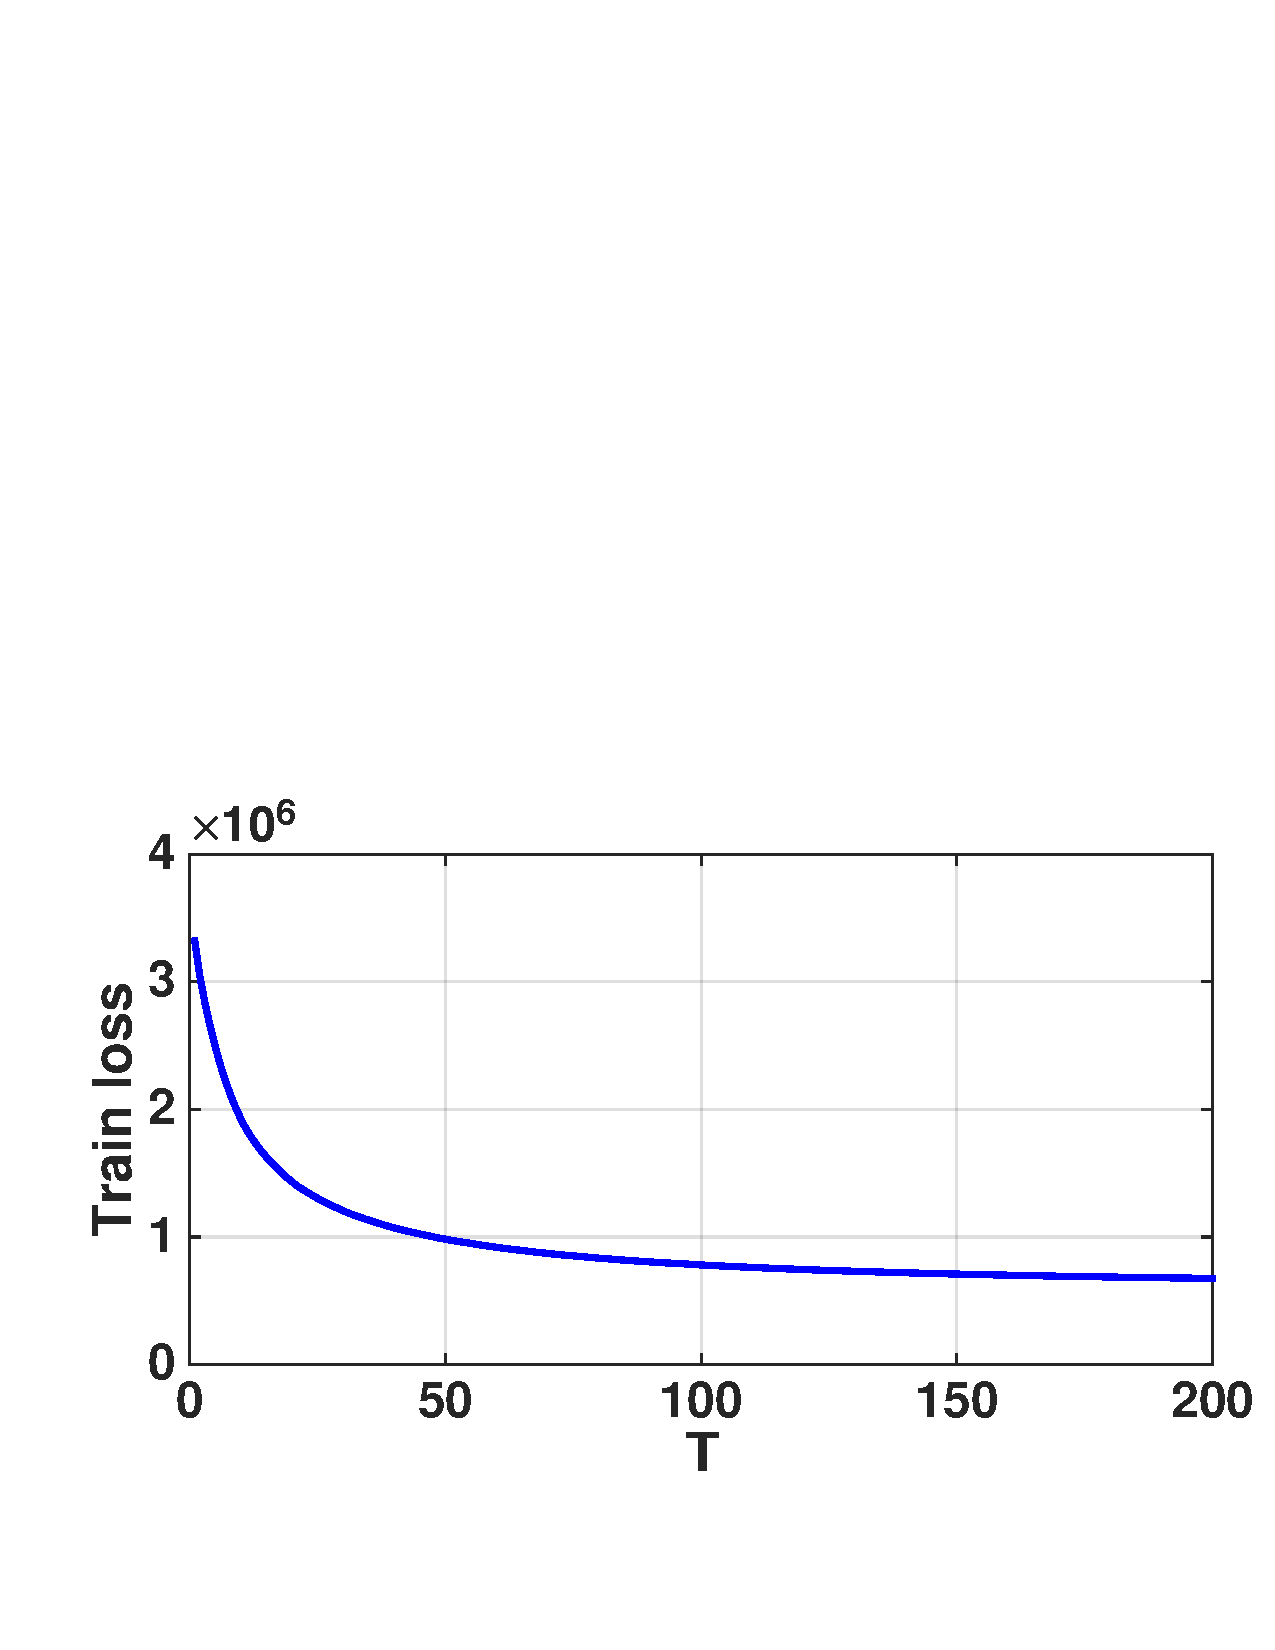
\includegraphics[width=4cm,height=2.35cm]{figures/four_train}}~~~
\subfigure [\emph{Foursquare} test loss]{ 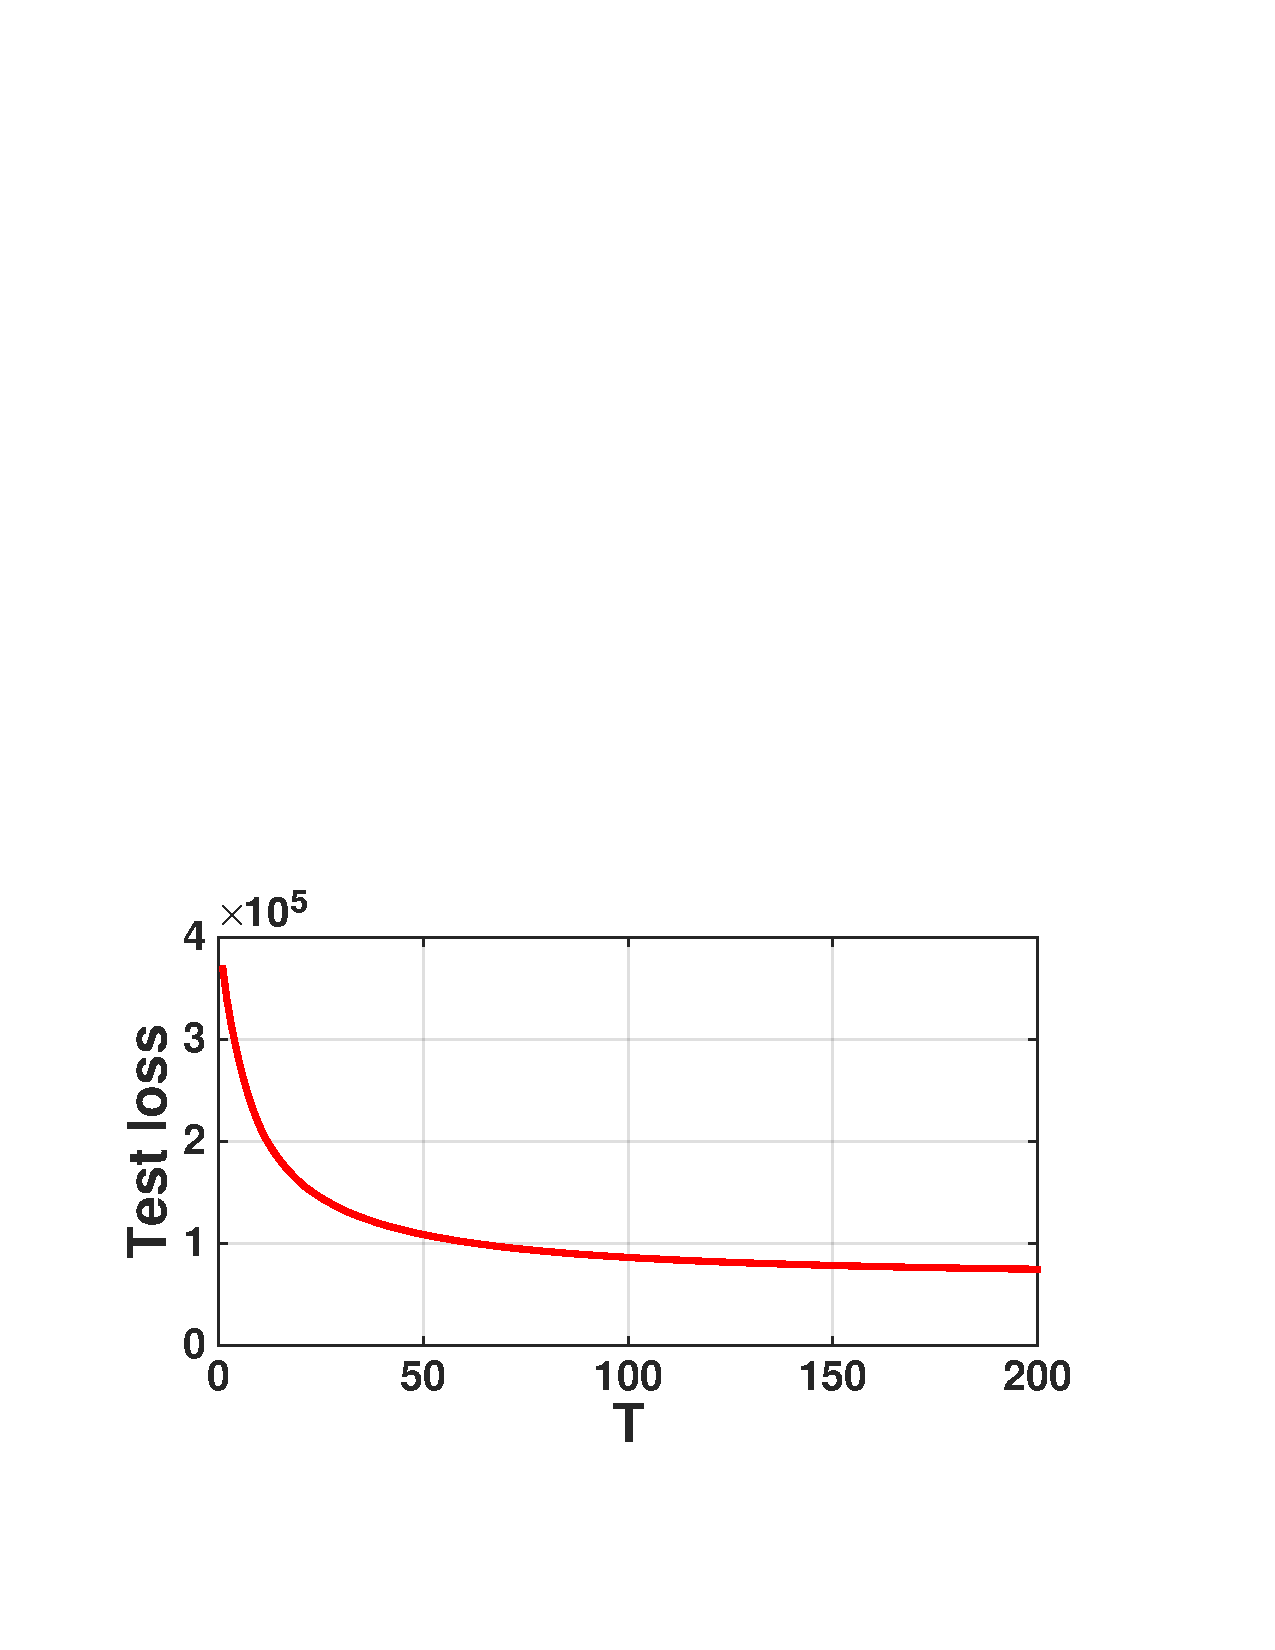
\includegraphics[width=4cm,height=2.35cm]{figures/four_test}}~~~
\subfigure [\emph{Alipay} training loss]{ 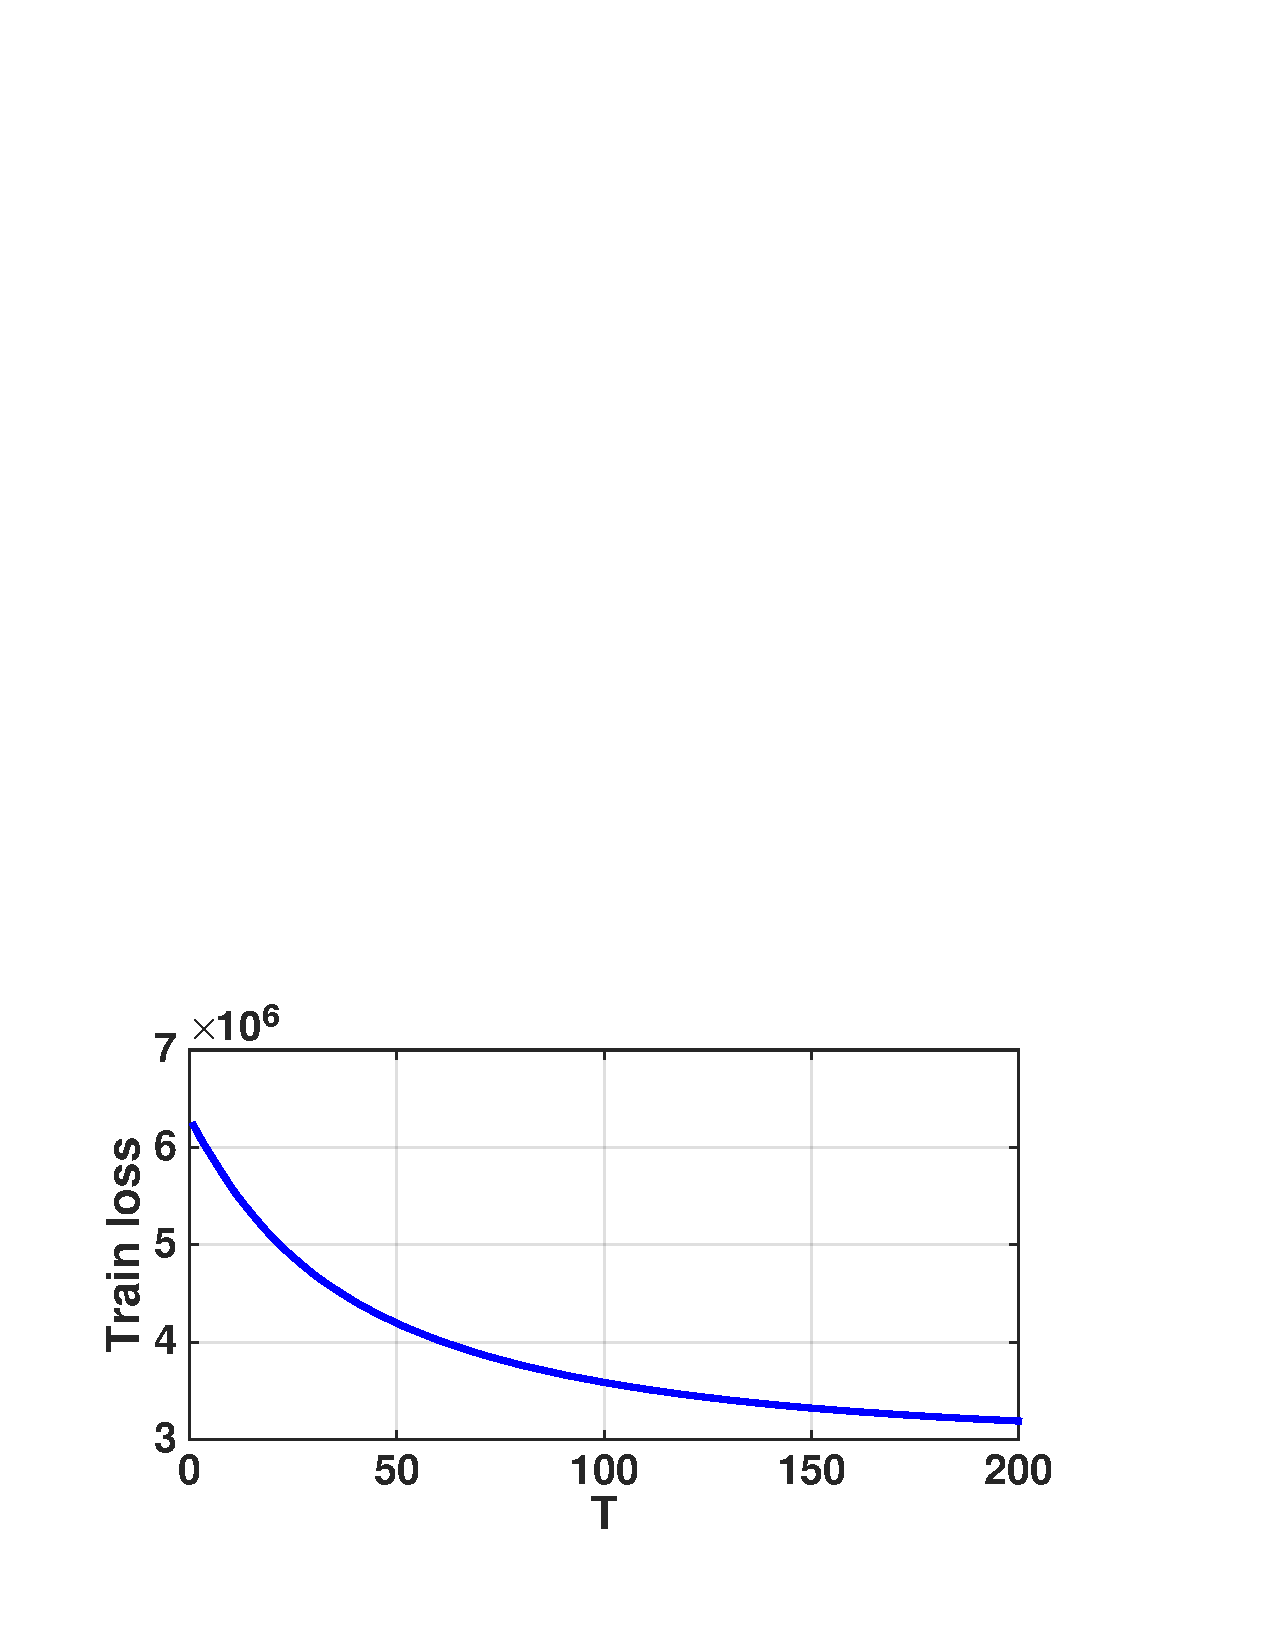
\includegraphics[width=4cm,height=2.35cm]{figures/alipay_train}}~~~
\subfigure[\emph{Alipay} test loss] { 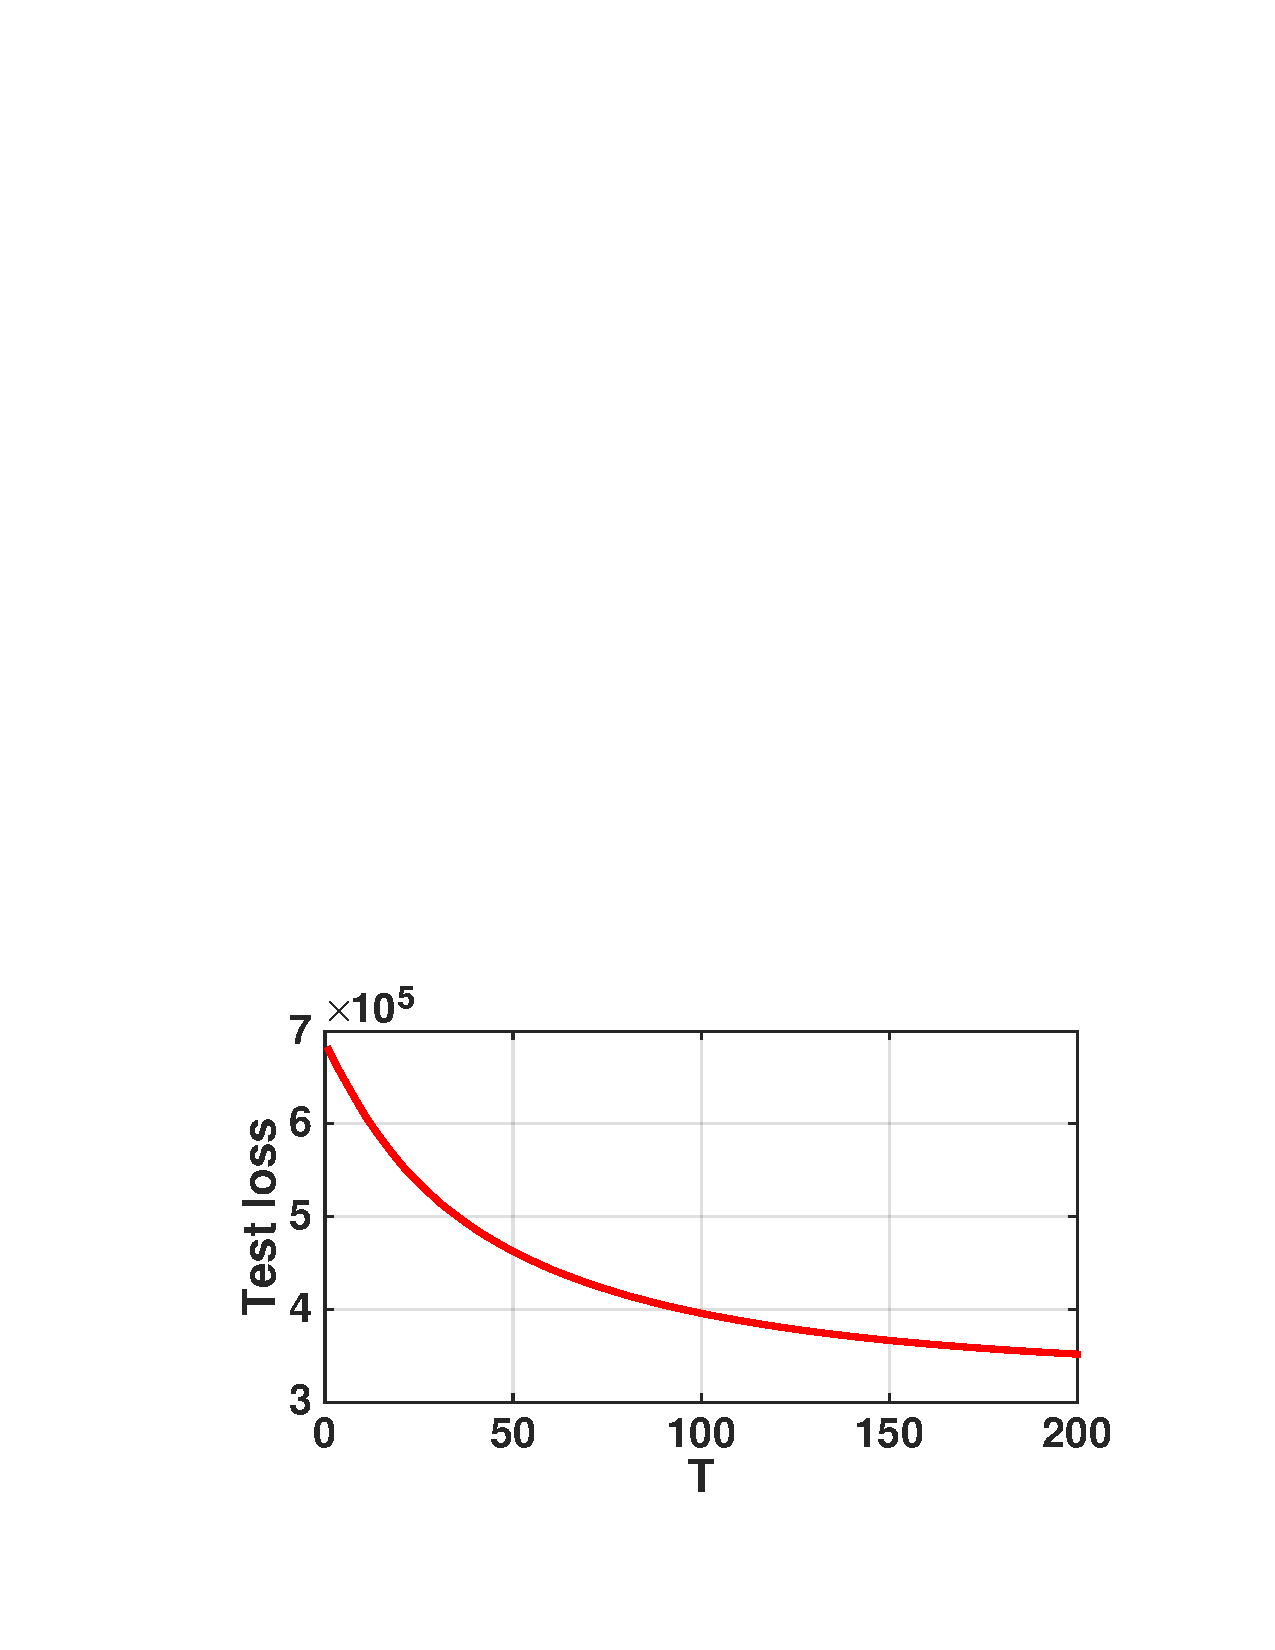
\includegraphics[width=4cm,height=2.35cm]{figures/alipay_test}}
\vskip -0.1in
\caption{The training and test loss of DMF with respect to the maximum iteration ($T$) on \emph{Foursquare} and \emph{Alipay} datasets. }
\label{effectoft}
%\vskip -0.15in
\end{figure*}

\begin{table}
\centering
\caption{Performance comparison on \emph{Alipay} dataset.}
%\vskip -0.1in
\label{Alipay}
\begin{tabular}{|c|p{1.15cm}<{\centering}|p{1.15cm}<{\centering}|p{1.15cm}<{\centering}|p{1.15cm}<{\centering}|}
 \hline
   Metrics & P@5 & R@5 & P@10 & R@10 \\
  \hline
  \hline
  Dimension & \multicolumn{4}{c|}{\emph{K=5}} \\
  \hline
  MF & 0.0209 & 0.0896 & 0.0134 & 0.1194 \\
  \hline
  BPR & 0.0243 & 0.1027 & 0.0166 & 0.1408 \\
  \hline
  GDMF & 0.0209 & 0.0937 & 0.0144 & 0.1231 \\
  \hline
  LDMF & 0.0017 & 0.0042 & 0.0008 & 0.0042 \\
  \hline
  DMF & \textbf{0.0267} & \textbf{0.1128} & \textbf{0.0228} & \textbf{0.1824} \\
  \hline
  \hline
  Dimension & \multicolumn{4}{c|}{\emph{K=10}} \\
  \hline
  MF & 0.0343 & 0.1493 & 0.0261 & 0.2239 \\
  \hline
  BPR & 0.0353 & 0.1512 & 0.0286 & 0.2439 \\
  \hline
  GDMF & 0.0304 & 0.1146 & 0.0277 & 0.2202 \\
  \hline
  LDMF & 0.0013 & 0.0065 & 0.0013 & 0.0131 \\
  \hline
  DMF & \textbf{0.0357} & \textbf{0.1612} & \textbf{0.0291} & \textbf{0.2537} \\
  \hline
  \hline
  Dimension & \multicolumn{4}{c|}{\emph{K=15}} \\
  \hline
  MF & 0.0378 & 0.1538 & 0.0266 & 0.2308 \\
  \hline
  BPR & \textbf{0.0448} & \textbf{0.1898} & 0.0342 & 0.2872 \\
  \hline
  GDMF & 0.0355 & 0.1383 & 0.0267 & 0.2123 \\
  \hline
  LDMF & 0.0137 & 0.0684 & 0.0103 & 0.0983 \\
  \hline
  DMF & 0.0413 & 0.1942 & \textbf{0.0370} & \textbf{0.3035} \\
  \hline
\end{tabular}
\end{table}

We report the comparison results on both \emph{Foursquare} and \emph{Alipay} datasets in Table \ref{Foursquare} and Table \ref{Alipay}, respectively. 
From them, we find that:
\begin{itemize}[leftmargin=*] \setlength{\itemsep}{-\itemsep}
    \item All the model performances increase with the dimension of latent factor ($K$). 
    %Take the result of DMF on \emph{Alipay} dataset for example, the $R@10$ performances of $K=10$ and $K=15$ improve that of $K=5$ by 22.95\% and 32.38\%, respectively. 
	This is because the latent factor with a bigger $K$ contains more information, and thus user and POI preferences can be learnt more precisely. 
	\item GDMF achieves comparable performance with MF, since users collaboratively learn the global item latent factor, which works similarly as the traditional MF. 
	\item LDMF behave the worst, since each user learn item preference only based on his own check-in data which is very sparse. This indicates the importance of user collaboration during recommendation. 
    %\item Our proposed nearby collaborative DMF (NCDMF) outperforms the classic MF model in almost all the cases. This is because, the classic centralized MF uses a single item latent matrix to denote the preferences of items, and on the contrary, each user has their own item latent matrix for NCDMF. Therefore, item preferences are more personalized in NCDMF, and they are learnt more precisely to match each user's favor. 
    \item DMF consistently outperforms MF, GDMF, and LDMF, and even beats the pairwise ranking model (BPR) in most cases. 
    Take the result of DMF on \emph{Alipay} dataset for example, $P@5$ and $R@5$ of DMF improve those of MF by 27.75\% and 25.89\% when $K=5$. 
    This is because, the item preference of DMF contains not only common preference that obtained from all the users' data, but also each user's  personal preference that learnt from his own data. 
    Moreover, the random walk technique intelligently help users to choose neighbors to communicate with. 
    Therefore, item preferences are learnt more precisely, to better match each user's favor. 
\end{itemize}

\subsection{Parameter Analysis}
Finally, we study the effects of parameters on DMF, including item global and local regularizer ($\beta$ and $\gamma$), maximum random walk distance ($D$), and maximum iteration ($T$). 


\textbf{Effect of $\beta$ and $\gamma$.} 

\begin{figure}[t]
\centering
\subfigure [\emph{Foursquare}]{ 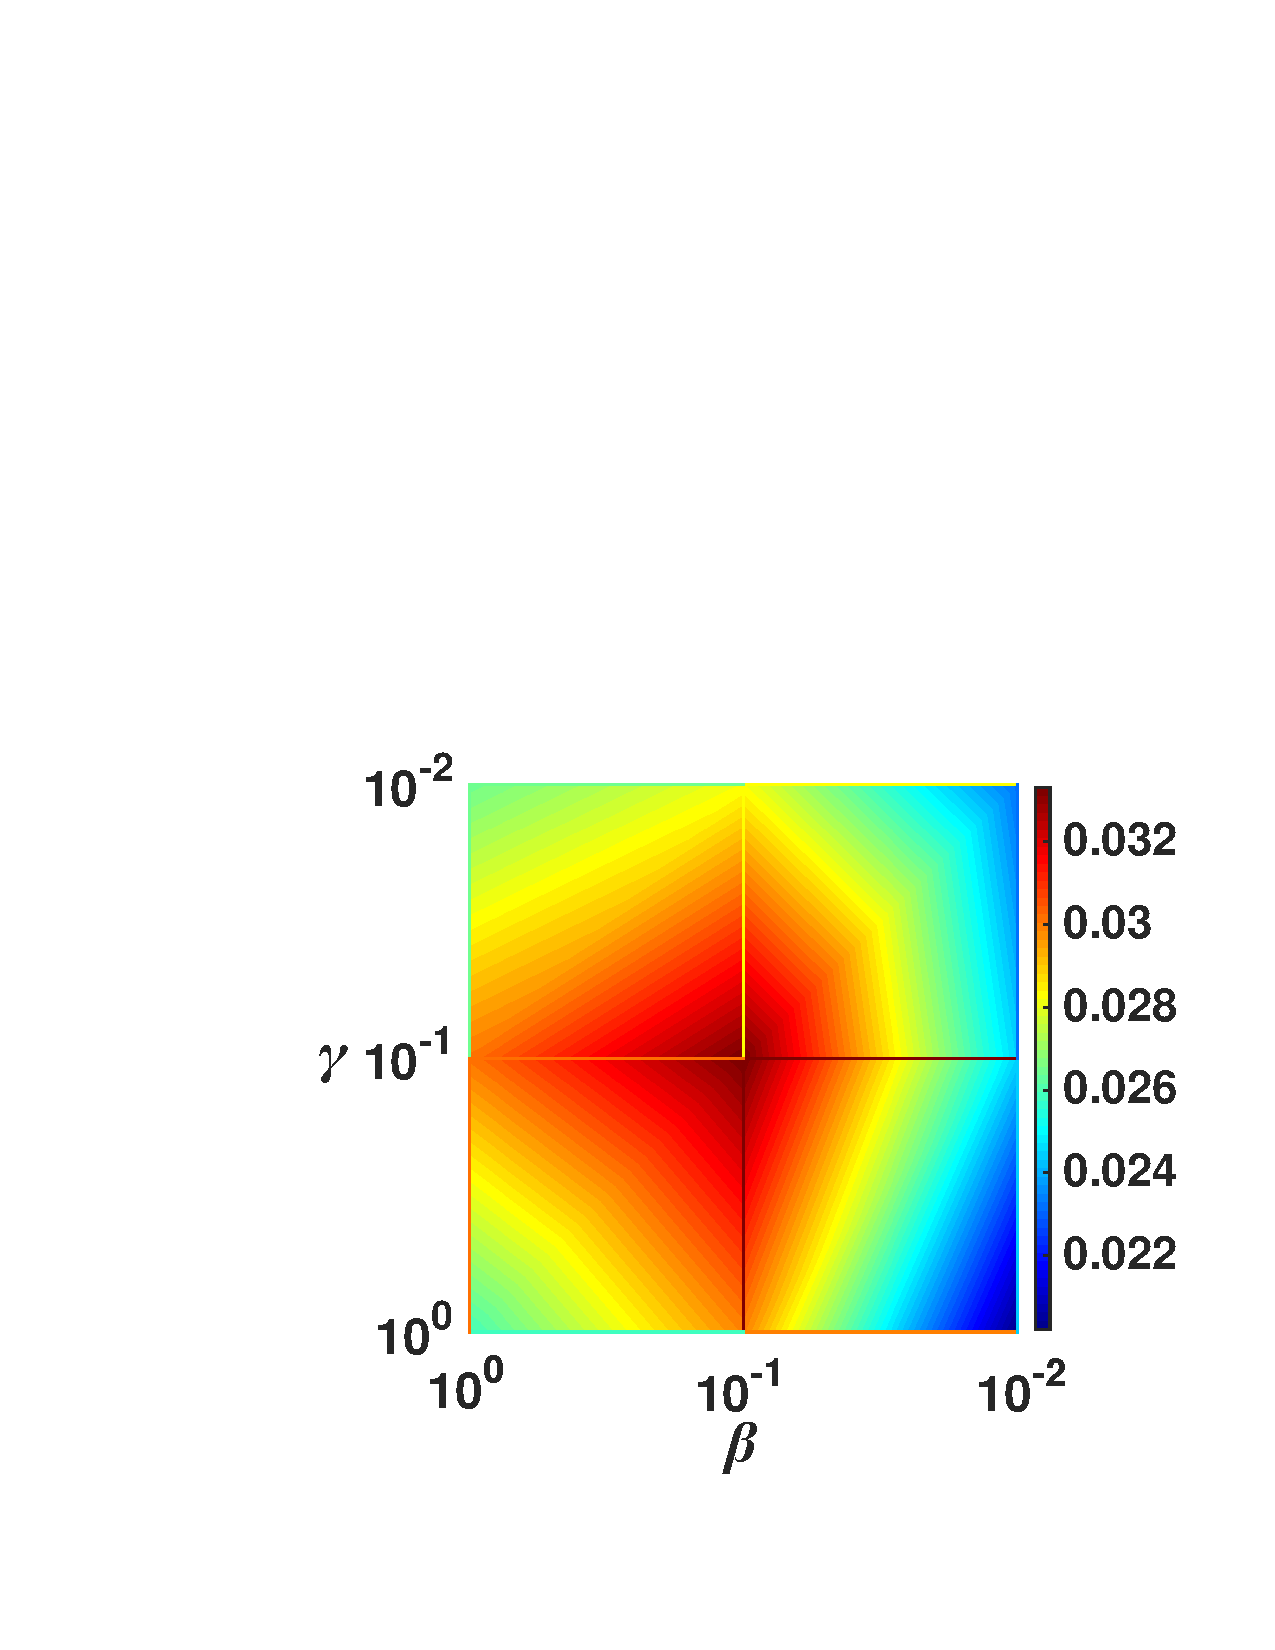
\includegraphics[width=4cm]{figures/four_l}}~~~
\subfigure[\emph{Alipay}] { 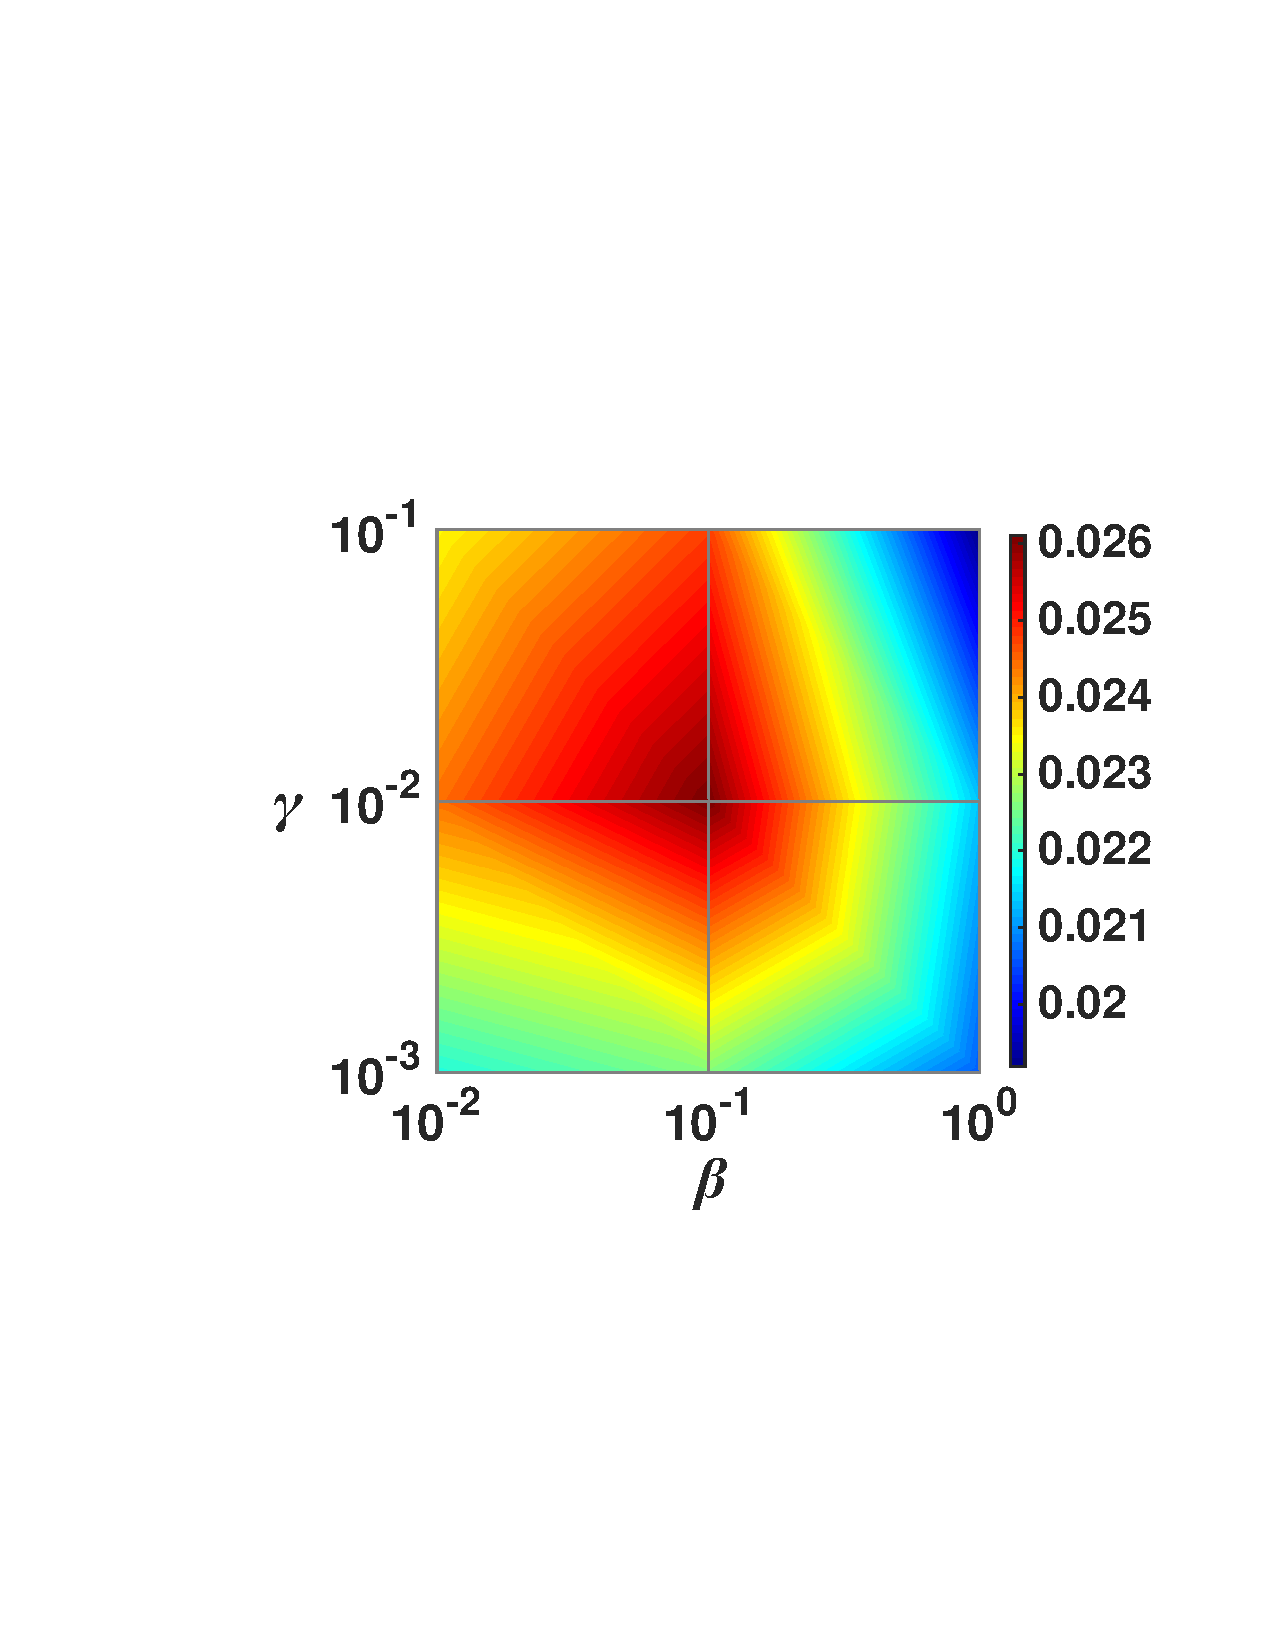
\includegraphics[width=4cm]{figures/alipay_l}}
\vskip -0.05in
\caption{Effect of $\beta$ and $\gamma$ on DMF. }
\label{effectofl}
%\vskip -0.15in
\end{figure}

The item global regularizer ($\beta$) and local regularizer ($\gamma$) controls the proportion of one's item preference comes from his own data or other users' data. 
The bigger $\beta$ is, the more one's item preference comes from his own data, and similarly, the bigger $\gamma$ is, the more one's item preference comes from other users' data through global item gradient (${\partial \mathcal{L}}/{\partial p^i_j}$) exchange. 
Figure \ref{effectofl} shows their effects on DMF on both datasets. 
From it, we can find that, with the good choices of $\beta$ and $\gamma$, DMF can make full use of one's own data and his neighbors' data, and thus, achieves the best performance. 

\textbf{Effect of maximum random walk distance ($D$).} 
The maximum random walk distance determinates how many neighbors will be communicated after a user has interaction with a POI, as we described in complexity analysis section. 
%The maximum number of neighbors to be communicated is $N^D$, where $N$ denotes the maximum number of directed neighbors of each user. 
Figure \ref{effectofd} shows its effect on DMF model on both \emph{Foursquare} and \emph{Alipay} datasets, where we set $K=5$ and fix other parameters to their best values. 
From it, we see that with the increase of $D$, our model performance increases, and tends to be relative stable when $D$ is bigger than 3. 
This shows that DMF achieves a good performance with only a small value of $D$, which indicates a low cost of communication complexity. 

\begin{figure}
\centering
\subfigure [\emph{Foursquare}]{ 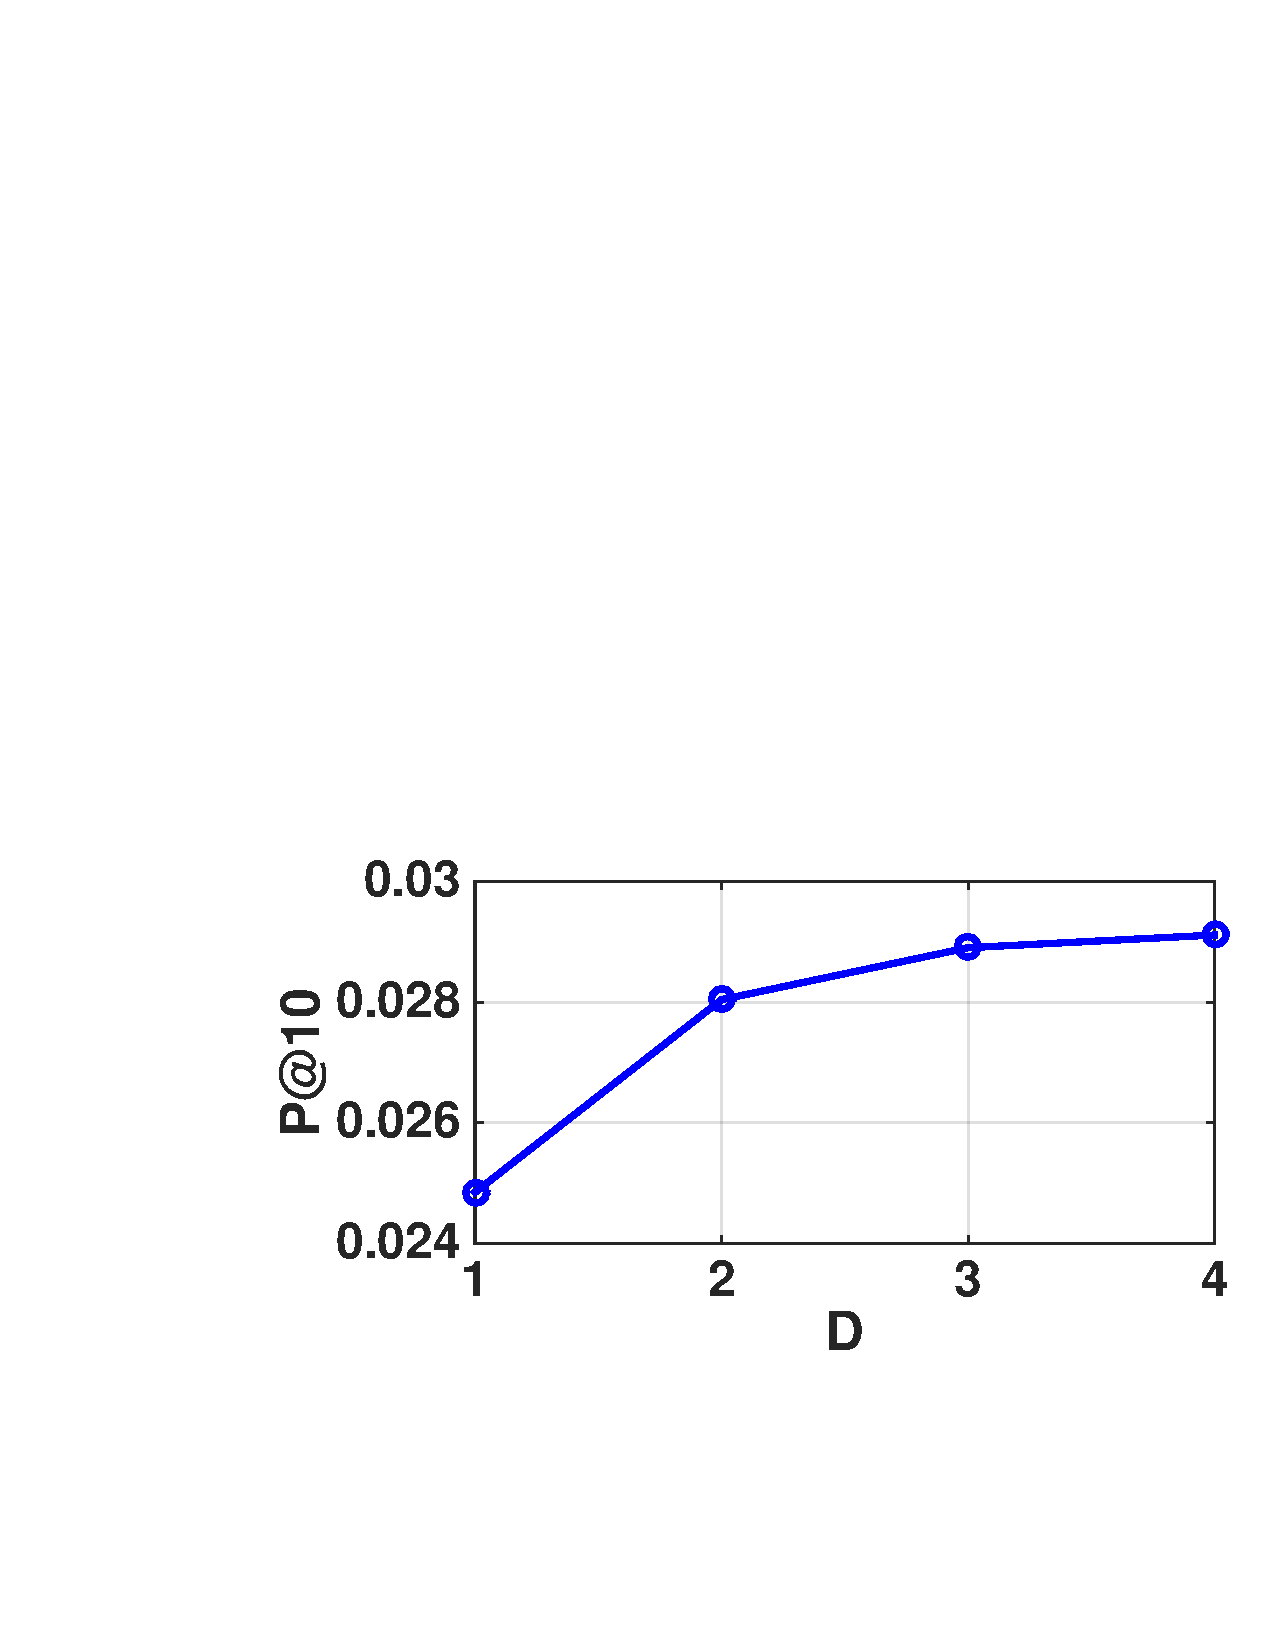
\includegraphics[width=4cm]{figures/four_d}}~~~
\subfigure[\emph{Alipay}] { 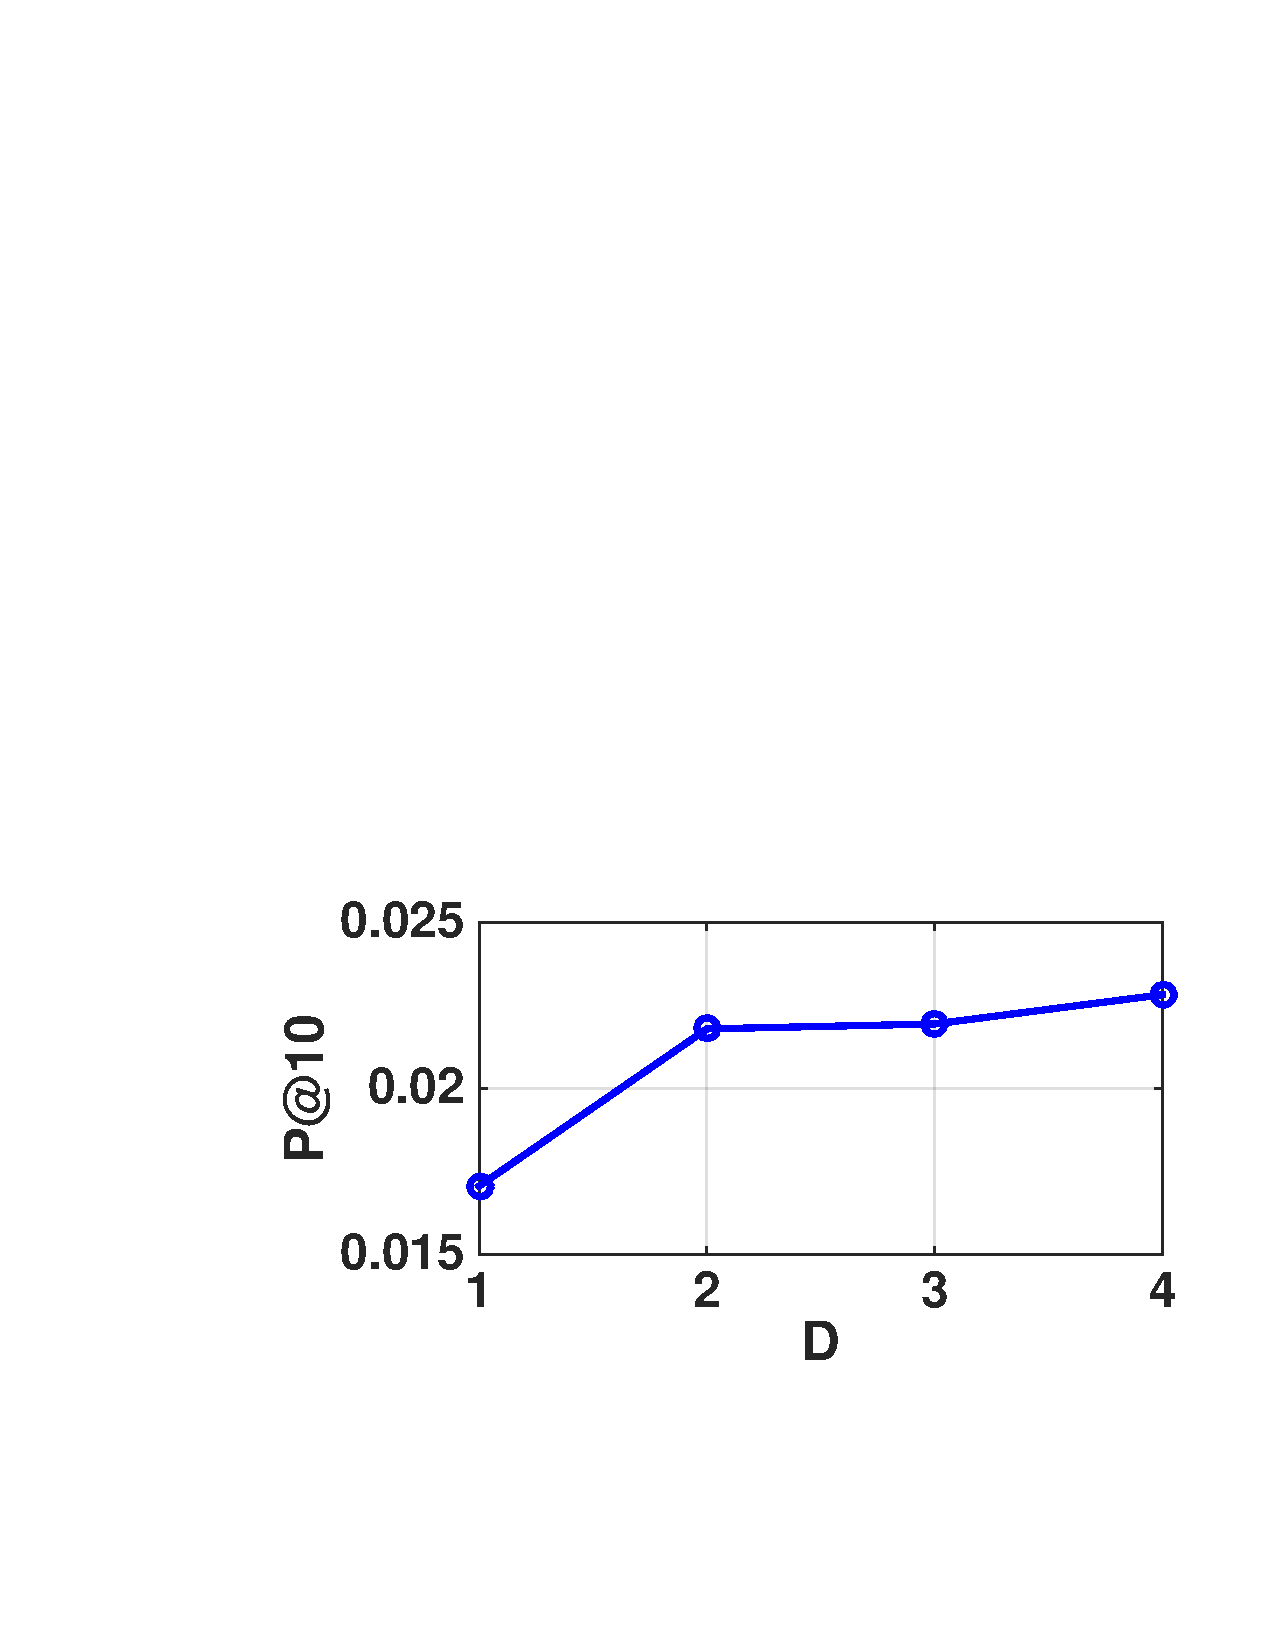
\includegraphics[width=4cm]{figures/alipay_d}}
\vskip -0.05in
\caption{Effect of $D$ on DMF. }
\label{effectofd}
\vskip -0.15in
\end{figure}

\textbf{Effect of maximum iteration ($T$).} 
As we analyzed above, the computing time complexity is linear with the training data size, and thus, the converge speed determines how long DMF should be trained. 
Figure \ref{effectoft} shows the effect of $T$ on training loss and test loss on both \emph{Foursquare} and \emph{Alipay} datasets. 
As we can observe, DMF converges steadily with the increase of $T$, and it takes about 100 epochs to converge on \emph{Foursquare} and about 200 epochs on \emph{Alipay}. 

